\chapter{Conclusion}
\label{sec:conclusion}

\section{Summary}

OpenCL is a free and open standard for general purpose parallel programming across various hardware devices. It is maintained by the Khronos Group and implemented by hardware vendors like NVIDIA, AMD or Intel. OpenCL is natively available for C and C++ although many wrappers for other languages exist. To use OpenCL in a C/C++ application an SDK is needed which contains the required header files (also available from Khronos) and static libraries. For running an application using OpenCL a corresponding driver has to be installed offering the API functions as well as a compiler to create kernels. Furthermore, one or more appropriate hardware devices supporting OpenCL are necessary and may even be used together.

The hardware architectures for which OpenCL can be used are quite different, especially concerning the differences between CPUs and GPUs.
Modern consumer CPUs have a small number of independent, high power cores (mostly four or eight) which can be used independently by an application using threads. Synchronization between the threads is easy and threads may be spawned at any time. High throughput can be achieved by distributing the work on all available cores and make use of vector instruction sets like SSE or AVX. Memory is provided as a large block behind a hierarchical cache system.

GPUs however employ a massive amount of less powerful cores (up to several thousands) packed together in multiprocessors. Work is processed in smaller work groups and larger n-dimensional ranges which often occupy hundreds or thousands of threads (which often have to be a multiple of hardware specific resources) executing the same code step by step. Synchronization is limited and the amount of threads used has to be predetermined every time work is offloaded to the GPU. High throughput is achieved by utilizing all components of the GPU (ALU, read and write units, etc.) as much as possible. Branching and synchronization should be avoided and vector types/operations should be used wherever possible to maximize the ALUs throughput. The large global memory is cached but very slow and sensitive concerning access patterns. Local memory is available as programmers-controlled cache but again suffers from misaligned accesses (bank conflicts). However, GPUs can achieve a much higher computational throughput than CPUs when used correctly.

Using OpenCL in an application starts by choosing an available platform/implementation and device. Additionally, a context and a command queue have to be created. Kernels are mostly created directly from their source code which has to be provided at run time. The source code is then compiled and linked into a program for the selected device and the kernels can be queried by name. To provide larger input and to retrieve output from a kernel, buffer objects have to be created. These may be read from and written to, either asynchronously or synchronously to the main application, by enqueuing operations on the command queue. Kernels are also enqueued and executed asynchronously after their arguments have been set.

To show the strengths and weaknesses of OpenCL and GPGPU computing on a few real world examples, three kinds of problems have been chosen for which various approaches have been implemented and benchmarked.

\begin{enumerate}
	\item
	At the beginning, multiplying two square matrices was ported to OpenCL. The CPU implementation is trivial but performs badly. Fortunately, highly tuned BLAS libraries exist which can do the multiplication a lot faster on the CPU. However, the first and again quite simple OpenCL implementation already beats the efficient BLAS sgemm routine. With some optimizations, making the code more complicated, we could push performance even further, achieving a speedup of 36.
	By the example of matrix multiplication we also took a look into performance analysis using profiler information from AMD's CodeXL.
	
	\item
	The second problem tackled was the all-prefix sum, a linear algorithm. The CPU implementation can be coded in a minute using a simple loop in a few lines of code. A naive, also quite easy to understand GPU approach performed fairly poor. By trying a more sophisticated tree-based reduce and scatter algorithm, small improvements could be made. Adding local memory and finally also using vector types and applying the algorithm on several layers in the end showed significant cut-downs on the run time (at the cost of hundreds of lines of code). However, the runtime of the CPU could not be beaten.
	
	\item
	The last implementation chapter focused one of the most famous topics in computer science, sorting. The two standard library routines \lstinline!qsort! and \lstinline!std::sort! have been benchmarked together with a radix sort implementation, the latter delivering amazing results. For sorting on the GPU, sorting networks have been introduced, because they are easy to parallelize. In particular, the bitonic sorter has been implemented and optimized. Despite the nasty input size restriction, the GPU implementation runs more than twice as fast as the comparison based variants on the CPU, which can be clearly seen as success. Radix sort, however, suffers from the GPUs highly parallel nature. Despite several optimizations it could not catch up and remains far behind the CPU implementation.
\end{enumerate}


\section{Conclusion}

In conclusion it can be said that GPUs are different from CPUs in the way they process work. This originates from their quite dissimilar hardware architectures as we discussed in the beginning. But not only the hardware itself, also the way algorithms have to be designed and programs have to be written differs largely from traditional single-thread-orientated CPU algorithms. Although it is already quite common to assign several tasks to several CPU cores (e.g., GUI and work thread), bringing parallelism down to small routines is still far from being common. When a program is designed to be run on massively parallel hardware we tend to spend more time on fighting with the peculiarities of the hardware than thinking about the actual problem we try to solve. This was one of the hardest challenges when implementing scan. The scan operation imposes high data dependency between the processed elements and therefore makes it perfectly suitable for as few processing units as possible. The GPU however benefits from a maximum of parallelism, on data and instruction level. Most of the time required to develop an efficient GPU scan was spent on trying to get enough parallelism on the cost of minimal redundancy in additions. Although the tree based approach worked well in the end, a lot of computing power is wasted during the up-sweep and down-sweep phase inside each work group. The same problem affected the radix sort GPU implementation. The per work item histogram was only required because the GPU does not ensure the order in which work items are processed. And to improve memory reading performance for the scan step by aligning the histogram buffer for coalesced access, the scattered, unblocked writes of the histograms at the end of the permute step also teared down performance, because GPUs profit enormously from reading and writing larger, consecutive blocks of memory. On the CPU, apart from worse caching, scattered accesses is less of a problem. The final argument, that should arise from this observations, is that programmers have to worry about a lot more different stuff than they have to when coding for a processor. Imagine Java or C\# programmers who are used to object-oriented design, dynamic memory allocation, huge standard libraries, containers and other complex data structures and all that candy of modern languages, when they find themselves porting one of their well-written, readable algorithms to the GPU where they have to break everything down into well-layouted arrays, think about the vectorizability of the produced instructions, repeatedly check the API documentation for a small number of built-in functions that might be of use and hunt down performance issues to stalled memory reads and bank conflicts. GPGPU computing is far different from modern software design and programming. Although the API is easily understood and the kernel language quickly learned, it takes months and probably years of practice to get a good feeling for designing GPU accelerated algorithms. GPUs are technological marvels offering immense computational power if used correctly. But it takes time to learn and study them in order to unfold their full potential.

Furthermore, it has to be said that not all algorithms fit the requirements of a GPU. In fact, only a small subset really benefits from the massively parallel hardware. In most cases, it is easier to focus on spreading a workload on several cores of the CPU instead of dealing with thousands of threads. Also the required memory transfer to and from the GPU is a crucial factor when deciding to offload a piece of work or not. If an algorithm does not fit the GPU one should not execute it there.

However, the small subset of algorithms which is often parallel in its nature may benefit tremendously from graphics hardware. We have discussed such a kind of algorithm on the example of multiplying matrices. The final speedup of 36 is amazing and shows the potential of GPU hardware when used at the right place.

So, when should OpenCL be used? Apart from having the right kind of algorithm to take advantage of GPGPU acceleration, also time and budget play an important role. Developing an algorithm for the GPU can be tedious and cumbersome and therefore time consuming. Furthermore, GPUs also impose a higher risk of failing to achieve the desired performance boost. The scan algorithms with optimizations may have taken two weeks to develop with the final outcome that the CPU variant is still faster. Experimenting with GPUs in a real world project should therefore be considered well, also concerning the aspect of system requirements. From a developers perspective, appropriate GPUs have to be available for implementing and testing and additional tools have to be installed for debugging and profiling. Concerning customers, appropriate hardware has to be available, drivers have to be installed and maybe the case of missing compatible hardware or drivers has to be handled (fallback CPU implementation). Talking about tools, the currently available suits from AMD (CodeXL), NVIDIA (Nsight, Visual Profiler) and Intel (SDK for OpenCL Applications) already provide decent help when developing software for their respective GPUs. However, they are still quite away from being as suitable and feature-rich as corresponding CPU debugger integration and profilers. Last but not least also maintainability and reusability play a vital role in modern software companies. Both aspects suffer in most cases as OpenCL algorithms tend to be optimized strongly to a specific kind of hardware and problem.

Finally, we have to see how long GPGPU computing will be done in this fashion. With the increasing power of on-chip GPUs on modern Intel processors, using GPUs for smaller tasks might become more attractive as no memory transfers will be required. AMD is also working intensively on a new generation of processing devices called Accelerated Processing Units (APU). By using a so-called heterogeneous system architecture (HSA), GPU and CPU are combined tightly on a single chip. The GPU will have direct access to the system's main memory with cache coherence to the CPU using the same address space as the CPU (theoretically allowing pointers to be passed). Furthermore, the GPU will allow multitasking via context switches between running tasks. As a result, long-running calculations will no longer freeze the display.
However, in another corner of the high performance hardware sector, Intel is heavily working on their new Many Integrated Core (MIC) architecture. The Intel Xeon Phi (previously named Knights Corner) is a co-processor card with up to 61 individual Intel processors and up to 16 GiB dedicated on-card memory. From an OpenCL programmers perspective, the Xeon Phi is equally programmed as a GPU. But the card is composed of modified x86 processors and can therefore also execute conventional software written in traditional languages. As a result, language integration is also easy. In fact, Intel's compiler already offers appropriate \lstinline!#pragma!s to offload parts of a C++ program to the co-processor card in a similar fashion as OpenMP. In addition, almost all drawbacks of GPUs vanish as all threads (four cores on each processor) can be fully synchronized, memory can be allocated dynamically on demand and all existing language features including libraries can be used. However, a Xeon Phi is still financially out of reach for consumers and still more expensive than decent GPUs with prices among several thousand dollars. But as time passes by, they may become affordable. Intel already announced that the next generation of the Xeon Phi (codename Knights Landing) will be capable of being used as the systems main processor. So maybe in ten years we find ourselves with a hundred main processors in our notebooks capable of handling even computationally expensive software with ease. Who needs GPU computing then?

\section{Personal experiences}

\subsection{Progress}

I began working on this thesis on 2012-07-23 by creating the code base for the sort project. Since then, 415 days have passed (today is the 2013-09-11). 436 commits have been made during this long period of time. The individual commit dates clearly mirror certain situations in my life at the time they were made. Figure \ref{fig:loc} presents how the lines of code have evolved over time, figure \ref{fig:commits} presents the commits made in this time.

\begin{figure}[h]
\centering
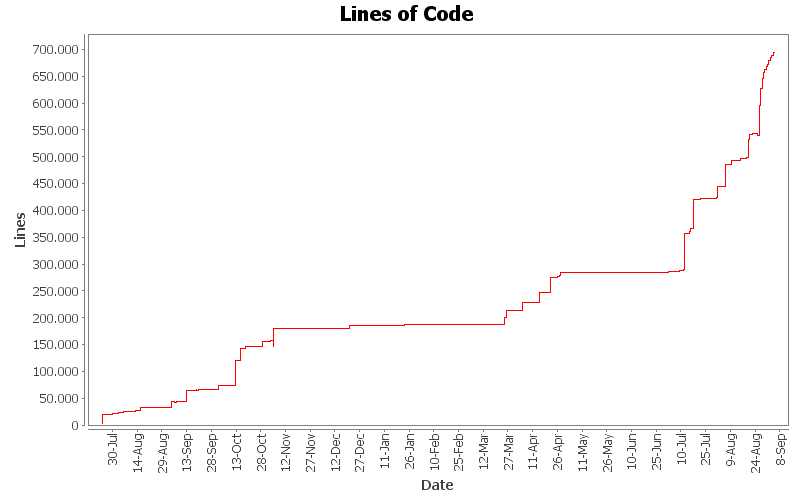
\includegraphics[width=0.9\textwidth]{loc}
\caption{Lines of code of all files in the repository over time. Chart generated using StatSVN.}
\label{fig:loc}
\end{figure}

\begin{figure}[h]
\centering
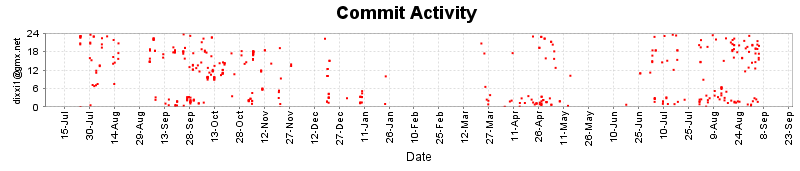
\includegraphics[width=0.9\textwidth]{commits}
\caption{My commits over time. Chart generated using StatSVN.}
\label{fig:commits}
\end{figure}

During the first days I worked intensively on setting up a comprehensive testing environment which should allow easy integration of new algorithms. At the beginning of my internship during the summer holidays in 2012, the commit dates started to occur in the morning (I tried to work two hours on this thesis before going to work), some at lunch time when I had come up with something during my work, but most of them in the late night. I soon realized an impact on my well-being from all the day and night programming and stopped working on my thesis several weeks later (cf. mid to late August in figure \ref{fig:commits}). However, my motivation for the internship also dropped and I had a bad conscience from showing no progress on my thesis. I quit my internship three weeks earlier to enjoy the remaining summer holidays and concentrate on the thesis. Fortunately, I could collect and integrate a lot of algorithms in this time from the beginning of September into the first weeks of university until the mid of October (cf. figure \ref{fig:commits}). Although I found less time from October to November due to studies, I could finish most of the code base and collected several benchmark data. My supervisor, FH-Prof. DI Dr. Heinz Dobler, and I were confident that I should be able to easily finish the thesis until February 2013, the first official data for handing in.

However, I made the mistake of accepting two tutorials (Programming and Project Engineering). Together with the increasing work load of my studies (mostly the large software projects by FH-Prof. DI Johann Heinzelreiter), I found almost no time to start writing. The two groups of commits around the 2012-11-20 and 2013-01-09 in figure \ref{fig:commits} were for the two presentations about the thesis in the bachelor seminar course. Apart from them, development was halted until the end of march, which is can be clearly seen in the advancement of the lines of codes in figure \ref{fig:loc}. After the end of the sixth semester at the end of March, I found again time to continue with my writing. I started to work on the introduction and OpenCL chapter.

I began my mandatory internship, which is part of the Software Engineering course, at the 2013-04-04. From the time of my commits during April in figure \ref{fig:commits} one can see that I was again writing on my thesis after work, sometimes until the morning hours. I found myself in the same situation as during my first internship during the summer, except there was no option to prematurely quit the internship. I was even working with the same technologies during work and at home. I lost most of my motivation and interest after a month and stopped working on my thesis after finishing the OpenCL chapter, which I sent to my supervisor. I also fought with bad health conditions, both physical and psychical.

I had the chance to learn a lot during my internship. However, as I was working with the same technologies as I use in my thesis, I came up with more and more design mistakes and ideas for improving my algorithms. During the last month of my internship, I felt the need to refactor most of the code produced during September and October 2012. This was the time where most of the final algorithms and sophisticated charts were created. By further tweaking the algorithms, I gathered a lot of in-depth knowledge about my implementations (which have mostly found their way into the matrix multiplication chapters). A finished my internship by the end of June, fortunately with amazing results and satisfied colleagues.

During the remaining time until the final deadline for the second bachelor exam (which is at the mid of September), I was working hard to write the implementation chapters. One of the big problems was the huge amount of information I had gathered around my implementations (mostly performance aspects). I was proud of all the peculiarities I found out about my GPU and how it behaves when processing my algorithms. However, time was of essence and I had to carefully decide on the algorithms and analyses to include. E.g., only the matrix multiplication contains a detailed view on performance counters. There was simply no time to include this kind of information in the other implementation chapters (although I would have loved to). Beside a week in France (the small gap around the end of July in figure \ref{fig:commits}) I used every day of my summer holidays for writing on my thesis. I finished the "Release Candidate" on 2013-08-25.

The remaining two weeks until the deadline, I was fully occupied with the creating of the second part of my thesis, which I surprisingly managed to finish during this time, producing an acceptable result. (Funny observation: During this time I also managed to change my sleep-wake cycle to more normal conditions, which can be seen at the commit times in figure \ref{fig:commits}). The last few days I was working on applying the feedback to my "Release Candidate".


\subsection{Positive and negative aspects}

Below is a list stating several positive (\ding{51}) and negative (\ding{55}) aspects encountered during the creation of this thesis:

\begin{itemize}
	 \item[\ding{51}] I started early with the implementation of my thesis at the beginning of my summer holidays in 2012.
	 \item[\ding{55}] I have selected to many subtopics/problems I wanted to cover in my thesis. It would probably have been a better idea to concentrate only on one problem (like matrix multiplication) and rename the thesis accordingly.
	
\end{itemize}













